\chapter{Példák}

\section{Sok körzőzés}
\begin{tikzExample}
    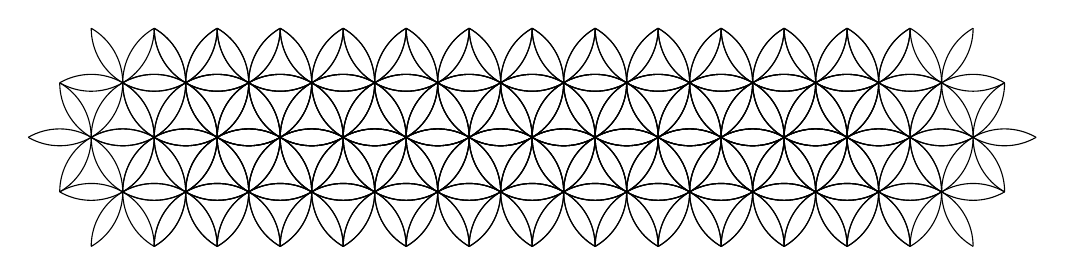
\begin{tikzpicture}[scale=0.8]
        \foreach \i in {0,...,12}
        {
            \draw (\i+0,0) circle (1);
            \draw (\i+0.5,-0.866) arc (0:120:1);
            \draw (\i+1.5,-0.866) arc (0:240:1);
            \draw (\i+-1,-0) arc (60:-60:1);
            \draw (\i+0,-1.732) arc (0:120:1);
            \draw (\i+-1.5,-0.866) arc (-120:120:1);
            \draw (\i+-1,-0) arc (-60:60:1);
            \draw (\i+-1.5,0.866) arc (-120:0:1);
            \draw (\i+0,1.732) arc (120:360:1);
            \draw (\i+0.5,0.866) arc (0:-120:1);
            \draw (\i+0.5,0.866) arc (-60:-180:1);
            \draw (\i+0.5,0.866) arc (120:240:1);
            \draw (\i+0.5,0.866) arc (180:300:1);
            \draw (\i+0.5,-0.866) arc (180:60:1);
            \draw (\i+-1,-1.732) arc (180:60:1);
            \draw (\i+1.5,0.866) arc (120:240:1);
            \draw (\i+0.5, 0.866) arc (0:60:1);
            \draw (\i+0.5, 0.866) arc (240:180:1);
            \draw (\i+0.5, 0.866) arc (240:300:1);
            \draw (\i+0.5, 0.866) arc (120:60:1);
            \draw (\i+0.5, 0.866) arc (180:120:1);
            \draw (\i+0.5, 0.866) arc (300:360:1);
            \draw (\i+-1,-0) arc (0:60:1);
            \draw (\i+-1,-0) arc (240:180:1);
            \draw (\i+-1,-0) arc (60:120:1);
            \draw (\i+-1,-0) arc (300:240:1);
            \draw (\i+-1,-0) arc (120:180:1);
            \draw (\i+-1,-0) arc (360:300:1);
            \draw (\i+0.5, -0.866) arc (180:240:1);
            \draw (\i+0.5, -0.866) arc (60:0:1);
            \draw (\i+0.5, -0.866) arc (120:60:1);
            \draw (\i+0.5, -0.866) arc (240:300:1);
            \draw (\i+0.5, -0.866) arc (120:180:1);
            \draw (\i+0.5, -0.866) arc (360:300:1);
        }    
    \end{tikzpicture}
\end{tikzExample}
    
\section{}
\begin{tikzExample}

\end{tikzExample}
